\documentclass[11pt, a4paper]{article}

\usepackage[spanish]{babel}
\usepackage[utf8]{inputenc}
\usepackage{graphicx}
\usepackage{caption}
\usepackage{subcaption}

% Margin set to a4wide
\usepackage{geometry}
\usepackage{layout}

\geometry{
  left=2.5cm,
  right=2.5cm,
  top=3.5cm,
  bottom=3cm
}

\usepackage{amsmath}
\usepackage{amstext}
\usepackage{amssymb}
\usepackage{hyperref}

\linespread{1.3}

\title{
    \large{Computación Paralela: Trabajo Final}\\
    \huge{Similitud Coseno Punto a Punto}
}

\author{Cristian A. Cardellino}

\date{12 de Agosto de 2015}

\begin{document}
  \maketitle

  \section{Introducción}

  El presente informe describe el trabajo final realizado para la cátedra de
  posgrado ``Computación Paralela''. El proyecto elegido fue la paralelización
  del algoritmo de {\em similitud coseno punto a punto} (pairwise cosine
  similarity) de una matriz.
  
  A grandes rasgos, el algoritmo toma una matriz y compara cada fila de esta
  contra todas las demás filas utilizando similitud coseno entre los vectores
  conformados por las filas. Luego devuelve una matriz de distancia con las
  distancias de cada par de filas en la matriz.

  La similitud coseno es una medida de la similitud existente entre dos
  vectores, en un espacio vectorial que posee producto punto, con el que se
  evalúa el valor del coseno del ángulo comprendido entre ellos. Esta medida
  proporciona un valor igual a 1 si el ángulo es cero, es decir ambos vectores
  apuntan al mismo lugar. Ante cualquier ángulo existente entre los vectores la
  medida arrojaría un valor menor a uno. En caso de vectores ortogonales la
  similitud es nula. Finalmente, si los vectores son opuestos, la medida sería
  -1.

  La similitud coseno puede ser aplicada a varias dimensiones, y es más
  comúnmente utilizada en espacios de alta dimensionalidad, e.g. búsqueda y
  recuperación de información (information retrieval) o minería de textos (text
  mining). 

  La similitud punto a punto es utilizada como técnica en sistemas de
  recomendación (recommender systems), particularmente en filtrado colaborativo
  (collaborative filtering), donde una matriz representa valoraciones
  (ratings) que ciertos usuarios les dan a ciertos items y esto a su vez es
  utilizado para recomendar dichos items a otros usuarios basándose en la
  similitud que tienen valorando items.

  La paralelización del presente problema se da en que la similitud entre dos
  filas de la matriz es completamente independiente por cada par de filas que
  haya en la matriz. No obstante, realizar este trabajo secuencialmente es del
  orden $\mathcal{O}(n^{2})$, donde $n$ es la cantidad de filas de la matriz.

  % TODO: Revisar outline
%  El informe se estructura de la siguiente manera: en la
%  Sección~\ref{sec:problema} se describe el problema particular sobre el que se
%  trabajaron las técnicas de optimización, se presentan los datos utilizados y
%  la manera en que se preprocesaron y como se representan dentro del problema;
%  la Sección~\ref{sec:experimentos} describe la configuración de los
%  experimentos, detalla el hardware utilizado en los mismos, se describe en
%  mayor detalle las distintas mejoras realizadas y los problemas con los
%  encontrados al realizarlas y se presentan las métricas y mediciones
%  utilizadas; la Sección~\ref{sec:resultados} muestra los resultados de los
%  experimentos y hace un análisis general de los mismos; finalmente el reporte
%  concluye en la Sección~\ref{sec:conclusiones}, donde se hace una observación
%  general del problema y los objetivos alcanzados.
 
  \section{Descripción del problema, datos y representación}\label{sec:problema}

  \subsection{Filtrado colaborativo basado en items}

  Los sistemas de recomendación (recommender systems) buscan predecir las
  preferencias de ciertos usuarios sobre ciertos items. En los últimos años se
  ha visto que estos sistemas se volvieron extremadamente comunes en distintas
  áreas como libros, películas, música, y productos en general. Grandes
  jugadores del medio del e-commerce o que brindan servicios de streaming hacen
  uso de estos sistemas para brindar una mejor experiencia de usuario (Netflix,
  Amazon, Spotify, entre otros).

  Dentro de estos sistemas, una técnica muy utilizada es el filtrado
  colaborativo (collaborative filtering) cuya idea parte de que usuarios
  similares tendrán gustos similares. El filtrado colaborativo es un método que
  busca hacer predicciones automáticas (filtrado) sobre los intereses de un
  usuario recolectando las preferencias de varios usuarios. La suposición que
  hace esta técnica es que si un usuario {\it A} tiene una opinión similar a un
  usuario {\it B} sobre determinado asunto, {\it A} es más probable que tenga
  una opinión similar a {\it B} en un asunto diferente a que tenga una opinión
  similar a algún otro usuario aleatorio {\it C}. Esto también es conocido como
  {\em filtrado colaborativo basado en usuarios} (user-based collaborative
  filtering) y tiene algunos problemas como:

  \begin{itemize}
    \item Bajo desempeño cuando hay muchos items pero pocas calificaciones.
    \item La cantidad de usuarios suele sobrepasar por varias magnitudes al
        número de items.
    \item Las preferencias de los usuarios pueden cambiar, lo que implica tener
        que recalcular todo el sistema.
  \end{itemize}

  Una variante de la técnica de filtrado colaborativo llamada {\em filtrado
  colaborativo basado en items}~\cite{linden2001collaborative} (item-based
  collaborative filtering) fue patentada por Amazon, y resuelve la mayoría de
  los problemas presentados por el filtrado basado en usuarios, particularmente
  en sistemas donde hay más cantidad de usuarios que de items. La idea base de
  esta técnica es recomendar items que sean similares a otros items que el
  usuario ya calificó positivamente, midiendo la similitud de dichos items. En
  este proyecto se busca paralelizar y optimizar el código básico que se usa
  para hacer este filtrado colaborativo basado en items.

  \subsection{Datos utilizados}\label{sec:datos}

  Para el desarrollo del proyecto se optó por datos estándar en la
  investigación de algoritmos de recomendación:
  MovieLens~\cite{Harper:2015:MDH:2866565.2827872}, de GroupLens Research. Este
  consta de distintas valoraciones (ratings) que usuarios del sitio web
  MovieLens\footnote{\url{http://movielens.org}} hicieron sobre distintas
  películas.

  GroupLens liberó distintos tamaños de su conjunto de datos para
  investigación. En este trabajo se hace uso de 4 de ellos:

  \begin{description} 
      \item[MovieLens 100k Dataset (ML100k)] Consta de 100000 valoraciones
          realizadas por 943 usuarios sobre 1682 películas.
      \item[MovieLens 1M Dataset (ML1M)] Consta de 1000209 valoraciones
          realizadas por 6040 usuarios sobre 3962 películas.
      \item[MovieLens 10M Dataset (ML10M)] Consta de 10000054 valoraciones
          realizadas por 69878 usuarios sobre 10677 películas.
      \item[MovieLens 20M Dataset (ML20M)] Consta de 20000263 valoraciones
          realizadas por 138493 usuarios sobre 26744 películas.
  \end{description}

  Las valoraciones de los usuarios están hechas en una escala de 5 estrellas
  (i.e. del rango [1, 5]), que en el caso de los datos de ML10M y ML20M pueden
  tener incrementos de media estrella (i.e., en el rango [0.5, 5.0]). Todos los
  conjuntos establecen que cada usuario valoró un mínimo de 20 películas.

  Los conjuntos ML100k y ML1M no tuvieron que ser modificados debido a que
  estos identificaron a sus películas y usuarios unívocamente con la cantidad.
  En el caso de los conjuntos ML10M y ML20M, estos tenían a sus usuarios y
  películas identificados con más números que la cantidad, por lo que se los
  preprocesó proyectando los valores de manera que estos fueran unívocos a la
  cantidad de usuarios/películas.

  \subsection{Representación de los datos}\label{sec:representaciones}

  Se requiere de dos archivos para hacer funcionar el código: la matriz de
  valoraciones y la matriz de similitud para corrección. La primera se obtuvo a
  partir de los datos brindados por MovieLens, la segunda se calculó utilizando
  la librería de aprendizaje automático de Python ``Scikit
  Learn''~\cite{scikit-learn}.

  La matriz de valoraciones contiene una fila por cada película y una columna
  por cada usuario del conjunto de datos.  Cada celda de la matriz representa
  la cantidad de estrellas que el usuario le dio a la película, siendo este
  valor igual a cero cuando el usuario no hizo valoración alguna sobre dicha
  película.

  Debido a que el conjunto de datos establece que cada usuario valoró un mínimo
  de 20 películas, dejando la mayoría de las películas sin valorar, la matriz
  final de películas/usuarios es extremadamente rala, llegando a ser los
  valores no nulos menor al 1\% de la totalidad de la matriz.

  En los primeros experimentos la matriz películas/usuarios era representada
  por una matriz densa. Sin embargo, era solo viable para los casos de los
  conjuntos ML100k y ML1M que se podía cargar dicha matriz en memoria sin que
  afectara gravemente el desempeño de los algoritmos encargados de calcular la
  similitud coseno. Buscando mejorar este desempeño para conjuntos de datos de
  mayor tamaño se optó por el uso de representaciones ralas para matrices; y
  dado que se necesita un acceso rápido a las filas para su comparación se hace
  uso del formato Yale (o {\em compressed row storage}) para representar las
  matrices.
  
  El archivo con el que se guarda la matriz de valoraciones sigue la base del
  formato de intercambio {\em Matrix Market}~\cite{Boisvert:aa}. Se usa el
  formato COO de matrices ralas coordinadas que durante la etapa de carga se
  transforma en formato Yale. 

  La matriz de corrección tiene la particularidad de ser una {\em matriz de
  distancia}, lo que quiere decir que es simétrica a través de la diagonal
  principal. Por lo tanto es suficiente con guardar la mitad triangular
  superior de la matriz. Para esto se hace uso de la propuesta de James D.
  McCaffrey: ``Converting a Triangular Matrix to an
  Array''\footnote{\url{https://jamesmccaffrey.wordpress.com/2010/05/14/converting-a-triangular-matrix-to-an-array/}}.

  \section{Optimizaciones}\label{sec:optimizaciones}

  \subsection{Algoritmo Base}

  El primer algoritmo, sin ninguna clase de optimización, es el que se busca
  mejorar en las instancias sucesivas de optimización.

  El algortimo comienza por cargar la matriz de ratings en su versión COO
  dentro de un arreglo utilizado como matriz de N filas por 3 columnas, donde N
  es el número de datos (en este caso ratings que posee el dataset) y en las 3
  columnas se almacena el valor de la fila (el ID de la película), el valor de
  la columna (el ID del usuario) y el rating. Esta es una representación
  sencilla de una matriz rala en formato COO.

  Si bien originalmente esta matriz era de enteros puesto que en los dos
  conjuntos de datos de menor tamaño (ml100k y ml1M, como se describe en la
  Sección~\ref{sec:datos}) los ratings eran únicamente valores enteros entre 1 y
  5. Sin embargo para los dos conjuntos de datos de mayor tamaño, los ratings
  podían tener ``media estrella'', por lo que los valores ya podían ser
  flotantes. Por esta razón, el arreglo pasó a ser de flotantes. 

  Se continúa con la carga del vector de corrección, que viene a ser el vector
  que representa la matriz de similitud coseno (como se describe en la
  Sección~\ref{sec:representaciones}) y que sirve como {\em gold standard} para
  asegurarse de que los cálculos se hicieron bien.

  El paso final de carga es el de la matriz de valoraciones, también descripta
  en la Sección~\ref{sec:representaciones}.  Esta será la matriz que se
  utilizará como base para los cálculos que se buscan optimizar. En los
  primeros experimentos esta matriz tiene una representación densa (a pesar de
  ser extremadamente rala).

  El algoritmo que se encarga del cálculo de la matriz de similitud coseno toma
  como entrada la matriz de valoraciones. El cálculo se realiza recorriendo
  cada par de filas (películas) una vez (puesto que la similitud entre la fila
  {\em i} y la fila {\em j} es la misma que la similitud entre la fila {\em j}
  y la fila {\em i}) y aplicando la {\em similitud coseno} entre los dos
  vectores que forman el par de filas.  En total, para recorrer todos los pares
  de filas de la matriz de valoraciones se necesitan
  $\frac{\text{P}^2+\text{P}}{2}$ iteraciones, donde P es el número de
  películas (o filas) de la matriz de valoraciones. Este valor es la dimensión
  final del vector que representa la matriz de similitud.

  La similitud coseno entre dos vectores \textbf{U} y \textbf{V} se define
  como:

  \[
      \text{cos\_sim}(\mathbf{U}, \mathbf{V}) = {\frac{\mathbf{U}\cdot\mathbf{V}}{\|\mathbf{U}\|\|\mathbf{V}\|}} = 
      {\frac {\sum \limits _{i=1}^{n}{U_{i}V_{i}}}{{\sqrt {\sum \limits _{i=1}^{n}{U_{i}^{2}}}}
      {\sqrt {\sum \limits _{i=1}^{n}{V_{i}^{2}}}}}}
  \]

  La sumatoria del numerador (num), la sumatoria del denominador para el vector
  \textbf{U} (uden), y la sumatoria del denominador para el vector \textbf{V}
  (vden), se realizan en el bucle que recorre cada par de filas. Luego, al
  final se almacena el valor de la similitud coseno dividiendo {\em num} por
  las raíces cuadradas de {\em uden} y {\em vden}. Este preocedimiento se
  repite durante algunas iteraciones para eliminar el ruido proveniente del uso
  de CPU para el cálculo. 

  El algoritmo finalmente compara la matriz de similitud (almacenada como un
  vector como se describe en la Sección~\ref{sec:representaciones}) con el
  vector de corrección cargado previamente.

  Por obvias razones este algoritmo es lento y se hace más y más difícil llegar
  a un resultado a medida que el tamaño del problema incrementa. Las primeras
  optimizaciones que se intentaron son con el uso de flags del compilador. No
  obstante sólo se probó el desempeño sin optimizaciones del compilador
  únicamente en el caso del conjunto de datos de menor tamaño (ml100k), puesto
  que cualquiera de los otros conjuntos hubieran terminado luego de demasiado
  tiempo y no aportarían nada al presente trabajo. Sólo las optimizaciones de
  compilación mejoraron el desempeño en aproximadamente {\bf 2.18x}.

  Hacer único el recorrido de cada par de filas fue también una mejora (obvia
  de realizar) con respecto a los primeros algoritmos donde se recorría cada
  par de filas existentes y no se discriminaban aquellos pares cuya conmutación
  había sido ya calculada. Además, en las primeras instancias también se
  utilizó una matriz densa para guardar los resultados de la matriz de
  similitud, lo que hacía que se duplicara la cantidad de valores a guardar
  (además de la memoria necesaria para estos).

  \subsection{OpenMP}

  Una optimización bastante sencilla de realizar sobre el cálculo en CPU era la
  paralelización en threads mediante OpenMP de los bucles que se encargan de
  recorrer los pares de filas de la matriz.

  Dado que cada par de filas posee una similitud coseno independiente de los
  demás pares y como cada par se recorre una sola vez (discriminando la
  conmutación de filas), esto era trivialmente paralelizable mediante el uso de
  un decorador \texttt{pragma omp parallel for}. Esto probó mejorar el
  desempeño en gran medida respecto a la versión base del algoritmo. Por
  supuesto, mientras más threads se usen, más rápido se obtienen los
  resultados.

  % TODO: Explicar la poca escalabilidad en eficiencia

  \subsection{CUDA}

  La siguiente optimización que se buscó sobre los cálculos fue mediante el uso
  de CUDA para paralelizar los cálculos via GPU. La base para cargar las
  matrices y vectores es la misma que en el caso de CPU. Por la naturaleza de
  CUDA, también hay que reservar los recursos necesarios en la GPU, además de
  hacer el traspaso de los datos desde la memoria del host a la memoria del
  device, lo que suma tiempo de cómputo.

  En CUDA, los kernels que se corren en paralelo son los encargados de un solo
  par de filas (películas) de la matriz. Se asegura mediante guardas
  condicionales que esto sea así para evitar condiciones de carrera. El
  algoritmo para hacer el cálculo es el mismo que en el caso que no se hace uso
  de GPUs, con algunas modificaciones como por ejemplo hacer uso de la función
  \texttt{rsqrt} para obtener las recíprocas de las raíces de los
  denominadores.

  Dado que necesitamos dos variables distintas en CUDA para recorrer la matriz
  (una por cada fila del par), los bloques de threads y del grid deben ser
  bidimensionales. De esta manera, una dimension se utiliza para identificar
  unívocamente una fila del par, mientras que la otra dimensión se utiliza para
  identificar la otra fila del par. Por esta razón, cada dimensión de los
  bloques no puede poseer más de 32 threads (de lo contrario sería de un total
  superior a 1024 threads por bloque). El tamaño de ambas dimensiones de la
  grilla, a su vez, se calcula de manera tal que se puedan procesar todas las
  filas de la matriz de similitud.

  CUDA muestra una mejora importante con respecto a la paralelización via CPU.

  \subsection{Matrices Ralas}

  La optimización final que se realiza sobre el problema original, y también la
  definitiva, es reemplazar la matriz de valoraciones por una representación
  rala de la misma. Esto mejora la performance tanto en velocidad como en
  memoria consumida.
  
  Dado que se busca realizar comparaciones por cada par de filas de la matriz,
  la mejor opción de representación de una matriz rala se encuentra en el
  formato Yale, también conocido como formato CRS (o Compressed Row Storage).
  La matriz se carga directamente desde el formato COO (que es con el formato
  que es guardada), al formato CSR, lo que elimina el proceso de convertir COO
  a una matriz densa.

  Para esta representación se tuvo que replantear la manera en que se calculaba
  la similitud coseno entre dos filas, puesto que la forma para matrices densas
  no funciona dado que no todas las filas tienen las mismas columnas para la
  representación rala de la matriz.

  En lugar de calcular el numerador y los denominadores en un mismo bucle
  \texttt{for}, se hace uso de tres bucles distintos: un bucle \texttt{while}
  para el cálculo del numerador y dos bucles \texttt{for} por separado para el
  caso de los denominadores. Esta fue la manera de evitar tener que pasar por
  muchas columnas en cada fila cuyos valores eran cero y no aportaban nada al
  resultado final.

  El caso del primer bucle, se optó por \texttt{while} porque era la forma de
  mantener control sobre que columna (o bien índice) de la fila se estaba
  realizando la operación de sumatoria. Y como esta es en sí un producto punto
  entre dos vectores ralos, solo tiene sentido que se sumen aquellos índices
  cuyo valor es distinto de cero.  Para el caso de los denominadores, se
  resolvió el cálculo por separado de cada denominador para sólo tener que
  recorrer las columnas en las que dicho denominador tenía valores no nulos.

  El valor final de la matriz de similitud sí se calcula de la misma manera que
  en los algoritmos anteriores.

  \section{Análisis de resultados}\label{sec:resultados}

  \subsection{Recursos de hardware}

  Se utilizó zx81 para realizar las mediciones de desempeño. El siguiente
  cuadro detalla los recursos de hardware de los que se dispusieron.

  \begin{table}[h]
      \centering
      \begin{tabular}{ll}
          \hline
          \textbf{CPU} & Intel(R) Xeon(R) CPU E5-2620 \\
          \textbf{Frecuencia} & 2.40 GHz \\
          \textbf{Cores} & 12 \\
          \textbf{Memoria} & 126 GiB \\
          \textbf{GPU} & NVIDIA GeForce GTX Titan \\
          \textbf{Memoria GPU} & 12 GiB \\
          \hline
      \end{tabular}
      \caption*{Recursos de hardware}
  \end{table}
 
  \subsection{Resultados}

  \subsubsection{Experimentos con OpenMP}

  Se realizaron varios experimentos haciendo uso de OpenMP para el cálculo de
  los datos. Para ver la escalabilidad de la paralelización con threads via
  CPU se probó realizar los experimentos con distinto número de threads.

  \begin{figure}[ht]
    \centering
    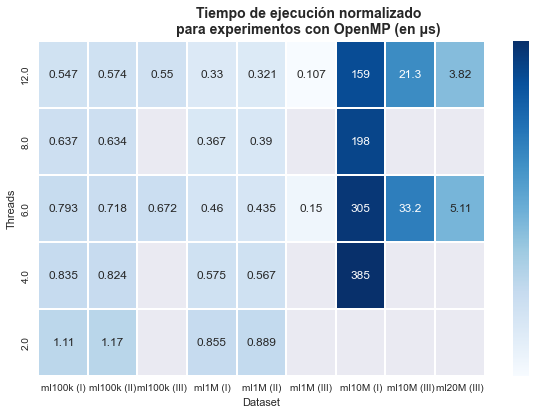
\includegraphics[width=\textwidth]{plots/heatmap_openmp.png}
      \caption{Heatmap de experimentos usando OpenMP}\label{fig:heatmap:omp}
  \end{figure}
 
  La Figura~\ref{fig:heatmap:omp} muestra los tiempos normalizados completos
  (i.e., el tiempo de cálculo sumado al tiempo de configuración) de distintos
  experimentos sobre los distintos conjuntos de datos, variando el número de
  threads con los cuales se corre OpenMP. Los tipos de experimentos que se
  detallan en la figura son los siguientes:

  \begin{description}
      \item[(I)] Ejecución con uso de matrices densas paralelizando un solo
          bucle \texttt{for} mediante el decorador \texttt{pragma omp parallel
          for}.
      \item[(II)] Ejecución con uso de matrices densas paralelizando ambos
          bucles \texttt{for} mediante el decorador \texttt{pragma omp parallel
          for}
      \item[(III)] Ejecución con uso de matrices ralas paralelizando un solo
          bucle \texttt{for} mediante el decorador \texttt{pragma omp parallel
          for}
  \end{description}
 
  La diferencia entre (I) y (II) se hizo para ver si el uso de dos decoradores
  que parelelizaran los bucles \texttt{for} anidados de la función de cálculo
  de la similitud coseno hacía alguna diferencia en los resultados finales
  (buscando como objetivo la escalabilidad). El experimento (II) sólo se llevó
  a cabo en los conjuntos de datos de menor tamaño (ml100k y ml1M) por una
  cuestión de practicidad, también es en estos conjuntos de menor tamaño que se
  realizaron experimentos con mayor cantidad de número de threads, debido a que
  en conjuntos de datos más grandes llevaría demasiado tiempo el cálculo
  utilizando poco número de threads.

  Para el caso de (III) ya se optó por sólo experimentar con la paralelización
  de un solo bucle \texttt{for} y para probar si con matrices ralas había mejor
  escalabilidad sólo se probó con 6 y 12 threads para ahorrar tiempo.

  El conjunto de datos ml10M se probó con matrices densas y ralas. En el caso
  de las matrices densas, como se explicó anteriormente, por cuestiones de
  practicidad sólo se experimentó haciendo uso de 4 o más threads. Es este
  conjunto el que arroja los peores resultados.

  Para el conjunto de datos de mayor tamaño (ml20M) sólo se pudo hacer
  experimentos utilizando matrices ralas, puesto que era imposible reservar
  memoria para matriz densa que se formaba para la matriz de valoraciones de
  este conjunto de datos.

  \subsubsection{Comparación de experimentos CUDA y OpenMP}
  
  \begin{figure}[ht]
    \centering
    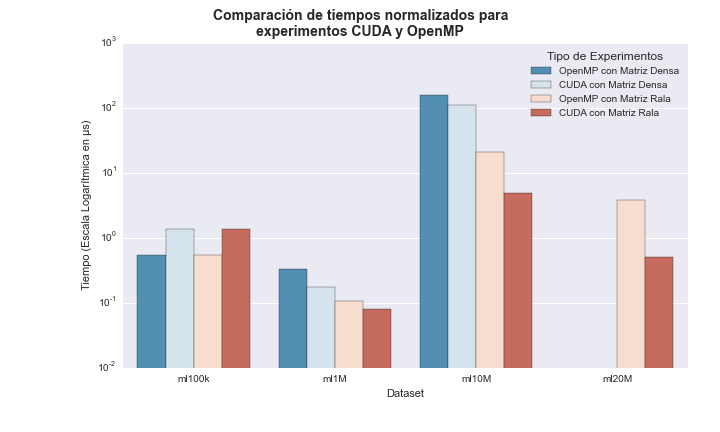
\includegraphics[width=\textwidth]{plots/cuda_omp.png}
      \caption{Comparación de experimentos CUDA y OpenMP}\label{fig:bar:cuda:omp}
  \end{figure}

  \begin{figure}[ht]
    \centering
    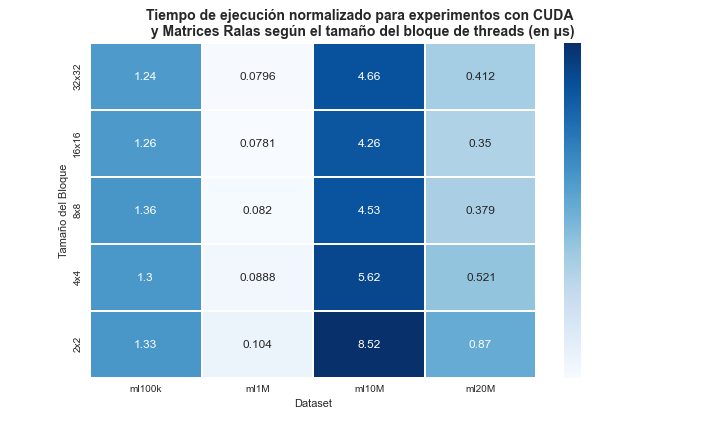
\includegraphics[width=\textwidth]{plots/cuda_sparse_blocks.png}
      \caption{Heatmap de experimentos usando CUDA}\label{fig:heatmap:cuda}
  \end{figure}

  \begin{figure}[ht]
      \centering
      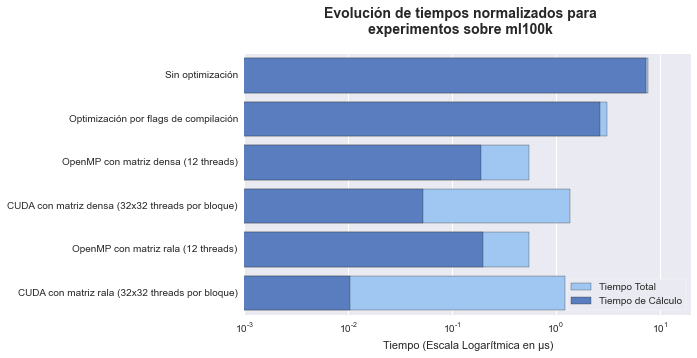
\includegraphics[width=\textwidth]{plots/ml100k.png}
      \caption{Evolución de tiempos sobre ml100k}\label{fig:ml100k}
  \end{figure}
 
  \begin{figure}[ht]
      \centering
      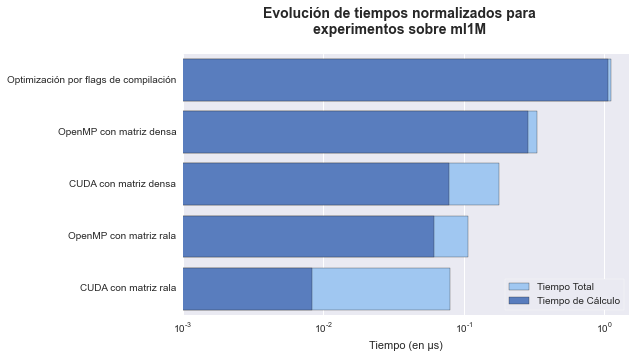
\includegraphics[width=\textwidth]{plots/ml1M.png}
      \caption{Evolución de tiempos sobre ml1M}\label{fig:ml1M}
  \end{figure}
 
  \begin{figure}[ht]
      \centering
      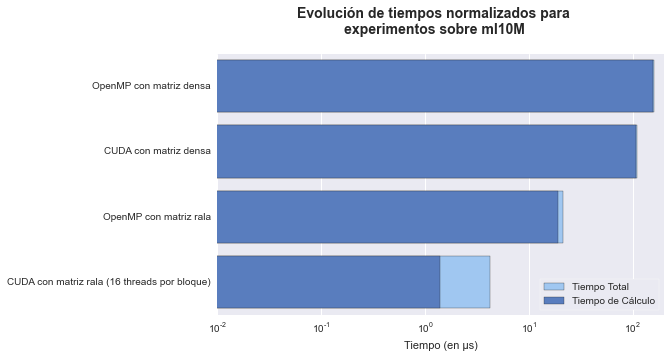
\includegraphics[width=\textwidth]{plots/ml10M.png}
      \caption{Evolución de tiempos sobre ml10M}\label{fig:ml10M}
  \end{figure}
 
  \begin{figure}[ht]
      \centering
      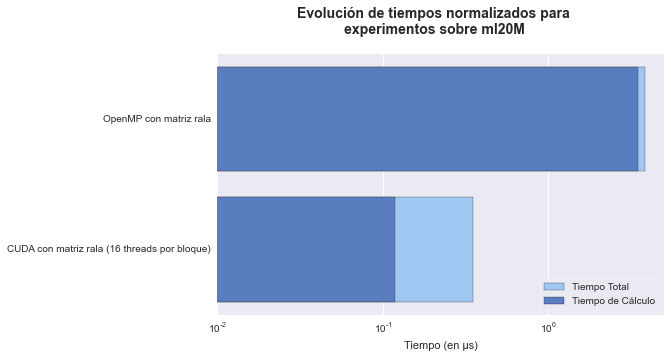
\includegraphics[width=\textwidth]{plots/ml20M.png}
      \caption{Evolución de tiempos sobre ml20M}\label{fig:ml20M}
  \end{figure}

  % Para 20M no se puede levantar la matriz. 3067 MiB el esparso.
  % Para 10M la matriz densa ocupa 6.2 GB en memoria. En sparse ocupa 659 MiB.

  % Gráficos: - Evolución final, desde el código en cero, sin optimización, hasta el código final. Sobre un dataset (100k)
  %         - Evolución de openmp respecto a los threads *
  %         - Comparación openmp con cuda (dense) en 12 threads (en teoría el mejor) *
  %         - Comparar sparse contra cuda y openmp en 12 threads *
  %         - Ver distintos valores de tamaño de bloque para sparse, solo GPU *

  % Ver resultados profiling mediante tabla (solo de los mejores valores): grpof, nvprof, perf

  \section{Conclusiones}\label{sec:conclusiones}

  \clearpage
  \bibliographystyle{abbrv}
  \bibliography{/Users/crscardellino/Documents/Posgrado/Bibliography/bibliography.bib}
\end{document}
